% ---------------------------------------------------------------------------
% Figura F3 — los cuatro controles del canal.  Bloque listo para pegar.
% NO insertado por la unidad: la inserción es de la autora.
%
% UBICACIÓN: capítulo del esquema, §3.5 «El procedimiento de validación», AL
% FINAL de la subsección, después del último párrafo — no en el medio, y no
% donde estaba el bloque de comentario [TODO: figura F3] de la versión vieja
% de §3.5 que todavía está en el repo.
%
% \includegraphics VA SIN EXTENSIÓN a propósito: pdflatex resuelve por su
% orden por omisión y toma figura_controles.pdf, el vectorial, con el texto
% como texto y sin depender de la resolución.  No hay PNG de esta figura.
%
% Sobre [H] y \linewidth: la figura mide 150 x 159,6 mm y su tipografía queda
% en 9,29 pt (títulos de control) y 8,18 pt (todo lo demás), MEDIDOS SOBRE EL
% PDF COMPILADO.  Con width=0.85\linewidth caerían a 7,90 / 6,95 pt, por
% debajo del piso de 8 pt: por eso la figura va a ancho pleno.
%
% Con el epígrafe, el bloque debería quedar del orden de 195 a 205 mm de los
% 257 mm de caja de texto (a4 menos los márgenes de 2 cm de main.tex:9), de
% modo que deja lugar para texto en su misma página.  ESTIMACIÓN NO
% VERIFICADA por compilación — no hay LaTeX en el entorno donde se generó la
% figura, así que conviene mirar la primera corrida.
% ---------------------------------------------------------------------------
\begin{figure}[H]
  \centering
  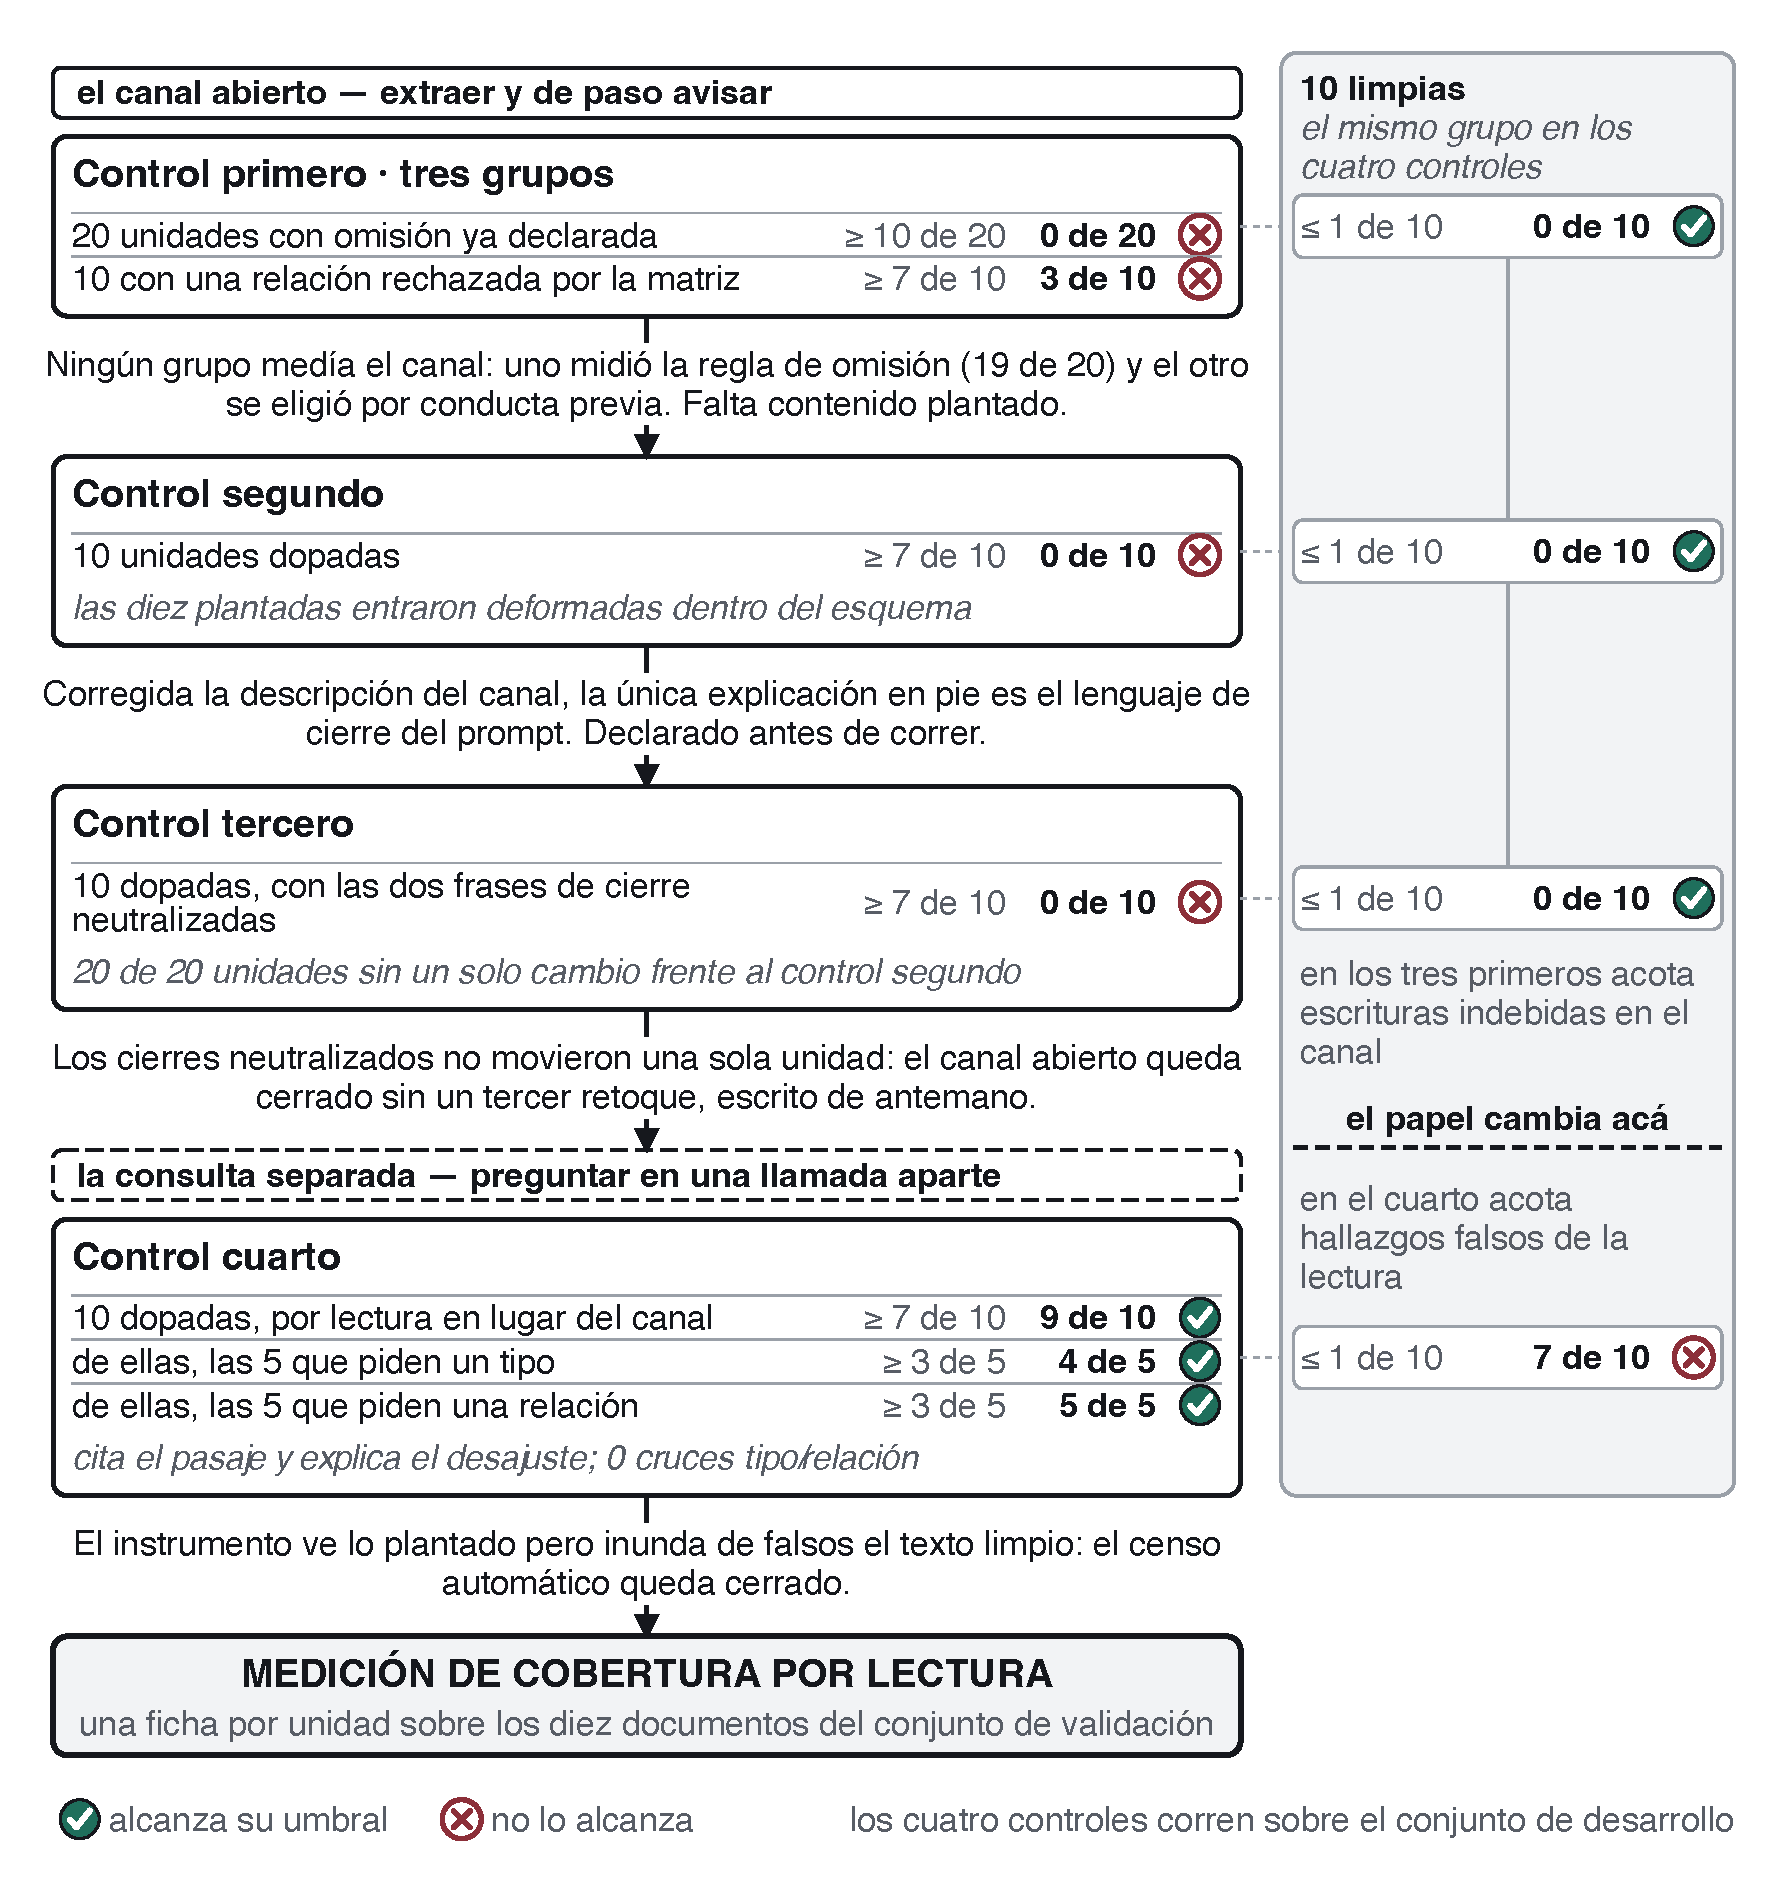
\includegraphics[width=\linewidth]{figuras/figura_controles}
  \caption[Los cuatro controles del canal]{Los cuatro controles, en el
    orden en que se corrieron. Sobre cada flecha va el motivo por el que
    hubo un control más, porque ninguno se corrió sin que el anterior
    fallara de una forma determinada. Los tres primeros prueban el canal
    abierto y el cuarto cambia de instrumento. El grupo de diez unidades
    limpias corre por la columna de la derecha y cambia de papel entre el
    tercer control y el cuarto, donde pasa de acotar escrituras indebidas
    en el canal a acotar hallazgos falsos de la lectura.}
  \label{fig:controles}
\end{figure}
